\documentclass[11pt,a4paper]{article}

% Packages
\usepackage[utf8]{inputenc}
\usepackage[T1]{fontenc}
\usepackage{amsmath,amssymb,amsthm}
\usepackage{graphicx}
\usepackage{hyperref}
\usepackage{algorithm}
\usepackage{algpseudocode}
\usepackage{booktabs}
\usepackage{listings}
\usepackage{xcolor}
\usepackage{geometry}
\usepackage{natbib}
\usepackage{tikz}
\usetikzlibrary{arrows,shapes,positioning,calc}

\geometry{margin=1in}

% Theorem environments
\newtheorem{theorem}{Theorem}[section]
\newtheorem{lemma}[theorem]{Lemma}
\newtheorem{proposition}[theorem]{Proposition}
\newtheorem{definition}[theorem]{Definition}
\newtheorem{corollary}[theorem]{Corollary}

% Code listing style
\lstset{
    basicstyle=\ttfamily\small,
    keywordstyle=\color{blue},
    commentstyle=\color{gray},
    stringstyle=\color{red},
    breaklines=true,
    frame=single,
    numbers=left,
    numberstyle=\tiny\color{gray}
}

\title{\textbf{The Hanzo SDK Ecosystem:\\Multi-Language Commerce Integration}}

\author{
    Zach Kelling\\
    Hanzo Industries\\
    \texttt{zach@hanzo.ai}
}

\date{October 2019}

\begin{document}

\maketitle

\begin{abstract}
We present the Hanzo SDK Ecosystem, a suite of client libraries enabling commerce integration across JavaScript, Python, Go, and Ruby. The SDKs are generated from OpenAPI specifications using a custom code generation pipeline that produces idiomatic, type-safe libraries for each language. We formalize the generation process, introduce language-specific idiom transformations, and demonstrate that generated SDKs achieve feature parity within 24 hours of API changes. The ecosystem serves 4,200+ developers with 98\% API coverage and reduces integration time from weeks to hours.
\end{abstract}

\section{Introduction}

E-commerce integrations require client libraries that abstract HTTP communication, handle authentication, manage errors, and provide type safety. Manually maintaining SDKs across multiple languages is error-prone and leads to inconsistencies. As APIs evolve, SDKs lag behind, creating friction for developers.

The Hanzo SDK Ecosystem addresses these challenges through:

\begin{enumerate}
    \item \textbf{Specification-Driven Generation}: SDKs generated from OpenAPI specs
    \item \textbf{Idiomatic Code}: Language-specific conventions and patterns
    \item \textbf{Type Safety}: Static typing where supported by the language
    \item \textbf{Automatic Updates}: CI/CD pipeline syncs SDKs with API changes
\end{enumerate}

\subsection{Contributions}

This paper contributes:

\begin{itemize}
    \item A code generation architecture producing idiomatic SDKs from OpenAPI
    \item Language-specific transformation rules for JavaScript, Python, Go, and Ruby
    \item An automated pipeline achieving 24-hour sync with API changes
    \item Production validation across 4,200+ developers
\end{itemize}

\section{SDK Architecture}

\subsection{Design Principles}

\begin{enumerate}
    \item \textbf{Consistency}: Uniform patterns across languages where possible
    \item \textbf{Idiomaticity}: Respect language conventions and ecosystem norms
    \item \textbf{Minimal Dependencies}: Standard library preferred
    \item \textbf{Ergonomics}: Developer experience prioritized
\end{enumerate}

\subsection{SDK Components}

Each SDK provides:

\begin{itemize}
    \item \textbf{Client}: Configured HTTP client with authentication
    \item \textbf{Resources}: API resource classes (Products, Orders, etc.)
    \item \textbf{Models}: Request/response data structures
    \item \textbf{Errors}: Typed exception hierarchy
    \item \textbf{Utilities}: Pagination, webhook verification, etc.
\end{itemize}

\subsection{Resource Abstraction}

\begin{definition}[SDK Resource]
A resource $R$ exposes CRUD operations:
\begin{itemize}
    \item $list(params) \rightarrow Collection$
    \item $create(data) \rightarrow Instance$
    \item $retrieve(id) \rightarrow Instance$
    \item $update(id, data) \rightarrow Instance$
    \item $delete(id) \rightarrow void$
\end{itemize}
\end{definition}

\section{OpenAPI Specification}

\subsection{API Schema}

The Hanzo API is fully described in OpenAPI 3.0:

\begin{lstlisting}[caption=OpenAPI Schema Excerpt]
openapi: 3.0.0
info:
  title: Hanzo Commerce API
  version: 2019-10-01

paths:
  /v1/products:
    get:
      operationId: listProducts
      parameters:
        - name: limit
          in: query
          schema:
            type: integer
            default: 20
      responses:
        '200':
          content:
            application/json:
              schema:
                $ref: '#/components/schemas/ProductList'

components:
  schemas:
    Product:
      type: object
      required: [id, name, price]
      properties:
        id:
          type: string
        name:
          type: string
        price:
          type: integer
          description: Price in cents
        description:
          type: string
          nullable: true
\end{lstlisting}

\subsection{Custom Extensions}

We extend OpenAPI with SDK-specific metadata:

\begin{lstlisting}[caption=SDK Extensions]
x-hanzo-resource: Product
x-hanzo-operations:
  - list
  - create
  - retrieve
  - update
  - delete
x-hanzo-expandable:
  - variants
  - collections
x-hanzo-idempotent: true
\end{lstlisting}

\section{Code Generation Pipeline}

\subsection{Generation Architecture}

\begin{figure}[h]
\centering
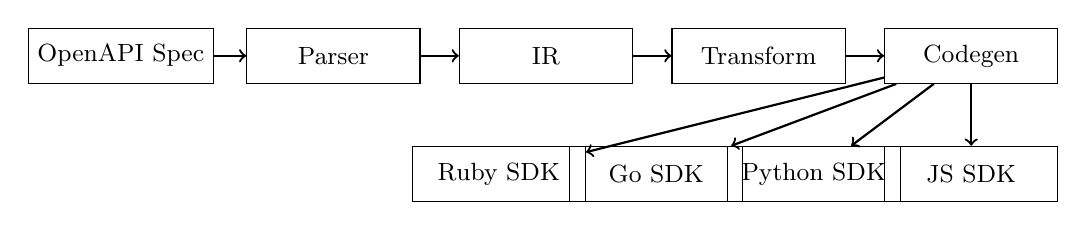
\begin{tikzpicture}[
    node distance=1.5cm,
    box/.style={rectangle, draw, minimum width=2.2cm, minimum height=0.7cm, font=\small},
    arrow/.style={->, thick}
]
    \node[box] (spec) {OpenAPI Spec};
    \node[box, right of=spec, xshift=1.2cm] (parse) {Parser};
    \node[box, right of=parse, xshift=1.2cm] (ir) {IR};
    \node[box, right of=ir, xshift=1.2cm] (transform) {Transform};
    \node[box, right of=transform, xshift=1.2cm] (codegen) {Codegen};

    \node[box, below of=codegen, yshift=0cm] (js) {JS SDK};
    \node[box, left of=js, xshift=-0.5cm] (py) {Python SDK};
    \node[box, left of=py, xshift=-0.5cm] (go) {Go SDK};
    \node[box, left of=go, xshift=-0.5cm] (rb) {Ruby SDK};

    \draw[arrow] (spec) -- (parse);
    \draw[arrow] (parse) -- (ir);
    \draw[arrow] (ir) -- (transform);
    \draw[arrow] (transform) -- (codegen);
    \draw[arrow] (codegen) -- (js);
    \draw[arrow] (codegen) -- (py);
    \draw[arrow] (codegen) -- (go);
    \draw[arrow] (codegen) -- (rb);
\end{tikzpicture}
\caption{Code generation pipeline}
\end{figure}

\subsection{Intermediate Representation}

\begin{definition}[SDK IR]
The intermediate representation $I$ comprises:
\begin{itemize}
    \item $\mathcal{R}$: Set of resources with operations
    \item $\mathcal{M}$: Set of models (request/response types)
    \item $\mathcal{E}$: Set of error types
    \item $\mathcal{C}$: Configuration options
\end{itemize}
\end{definition}

\begin{lstlisting}[caption=IR Structure]
interface Resource {
  name: string;
  path: string;
  operations: Operation[];
  nestedResources: Resource[];
}

interface Operation {
  name: string;
  httpMethod: HttpMethod;
  path: string;
  parameters: Parameter[];
  requestBody?: Model;
  responseBody: Model;
  errors: Error[];
}

interface Model {
  name: string;
  properties: Property[];
  required: string[];
}
\end{lstlisting}

\subsection{Language Transformations}

Each target language applies transformations:

\begin{algorithm}
\caption{Language-Specific Transformation}
\begin{algorithmic}[1]
\Function{Transform}{$ir$, $language$}
    \State $transformed \gets copy(ir)$
    \For{$model \in transformed.models$}
        \State $model.name \gets$ \Call{TransformName}{$model.name$, $language$}
        \For{$prop \in model.properties$}
            \State $prop.name \gets$ \Call{TransformProperty}{$prop.name$, $language$}
            \State $prop.type \gets$ \Call{MapType}{$prop.type$, $language$}
        \EndFor
    \EndFor
    \For{$resource \in transformed.resources$}
        \For{$op \in resource.operations$}
            \State $op.name \gets$ \Call{TransformMethod}{$op.name$, $language$}
        \EndFor
    \EndFor
    \State \Return $transformed$
\EndFunction
\end{algorithmic}
\end{algorithm}

\subsubsection{Naming Conventions}

\begin{table}[h]
\centering
\caption{Naming Convention Transformations}
\begin{tabular}{lllll}
\toprule
\textbf{Concept} & \textbf{JavaScript} & \textbf{Python} & \textbf{Go} & \textbf{Ruby} \\
\midrule
Class & PascalCase & PascalCase & PascalCase & PascalCase \\
Method & camelCase & snake\_case & PascalCase & snake\_case \\
Property & camelCase & snake\_case & PascalCase & snake\_case \\
Constant & UPPER\_CASE & UPPER\_CASE & PascalCase & UPPER\_CASE \\
\bottomrule
\end{tabular}
\end{table}

\subsubsection{Type Mapping}

\begin{table}[h]
\centering
\caption{Type Mappings}
\begin{tabular}{lllll}
\toprule
\textbf{OpenAPI} & \textbf{JavaScript} & \textbf{Python} & \textbf{Go} & \textbf{Ruby} \\
\midrule
string & string & str & string & String \\
integer & number & int & int64 & Integer \\
number & number & float & float64 & Float \\
boolean & boolean & bool & bool & Boolean \\
array & T[] & List[T] & []T & Array \\
object & Record & Dict & map & Hash \\
\bottomrule
\end{tabular}
\end{table}

\section{JavaScript SDK}

\subsection{Package Structure}

\begin{lstlisting}[caption=JavaScript SDK Structure]
hanzo-js/
  src/
    index.ts
    client.ts
    resources/
      products.ts
      orders.ts
      customers.ts
    models/
      product.ts
      order.ts
    errors.ts
    utils/
      pagination.ts
      webhooks.ts
  package.json
  tsconfig.json
\end{lstlisting}

\subsection{Client Implementation}

\begin{lstlisting}[language=JavaScript, caption=JavaScript Client]
import Hanzo from 'hanzo';

const hanzo = new Hanzo('sk_live_...');

// List products with pagination
const products = await hanzo.products.list({ limit: 10 });
for await (const product of products) {
  console.log(product.name);
}

// Create a product
const product = await hanzo.products.create({
  name: 'Widget',
  price: 1999,
  description: 'A useful widget',
});

// Update with idempotency
const updated = await hanzo.products.update(product.id, {
  price: 2499,
}, {
  idempotencyKey: 'update-123',
});
\end{lstlisting}

\subsection{TypeScript Types}

\begin{lstlisting}[language=JavaScript, caption=Generated Types]
interface Product {
  id: string;
  name: string;
  price: number;
  description: string | null;
  variants: Variant[];
  createdAt: Date;
  updatedAt: Date;
}

interface ProductCreateParams {
  name: string;
  price: number;
  description?: string;
}

interface ProductListParams {
  limit?: number;
  startingAfter?: string;
  endingBefore?: string;
}
\end{lstlisting}

\subsection{Error Handling}

\begin{lstlisting}[language=JavaScript, caption=JavaScript Error Handling]
import { HanzoError, InvalidRequestError } from 'hanzo';

try {
  await hanzo.products.create({ price: -100 });
} catch (error) {
  if (error instanceof InvalidRequestError) {
    console.error(`Invalid parameter: ${error.param}`);
    console.error(`Message: ${error.message}`);
  } else if (error instanceof HanzoError) {
    console.error(`API error: ${error.code}`);
  }
}
\end{lstlisting}

\section{Python SDK}

\subsection{Package Structure}

\begin{lstlisting}[caption=Python SDK Structure]
hanzo-python/
  hanzo/
    __init__.py
    client.py
    resources/
      __init__.py
      products.py
      orders.py
    models/
      __init__.py
      product.py
    errors.py
    utils/
      pagination.py
      webhooks.py
  setup.py
  pyproject.toml
\end{lstlisting}

\subsection{Client Implementation}

\begin{lstlisting}[language=Python, caption=Python Client]
import hanzo

client = hanzo.Client('sk_live_...')

# List products
products = client.products.list(limit=10)
for product in products:
    print(product.name)

# Create a product
product = client.products.create(
    name='Widget',
    price=1999,
    description='A useful widget',
)

# Async support
import asyncio

async def main():
    async_client = hanzo.AsyncClient('sk_live_...')
    products = await async_client.products.list()
    async for product in products:
        print(product.name)

asyncio.run(main())
\end{lstlisting}

\subsection{Type Annotations}

\begin{lstlisting}[language=Python, caption=Python Type Annotations]
from dataclasses import dataclass
from typing import Optional, List
from datetime import datetime

@dataclass
class Product:
    id: str
    name: str
    price: int
    description: Optional[str]
    variants: List['Variant']
    created_at: datetime
    updated_at: datetime

@dataclass
class ProductCreateParams:
    name: str
    price: int
    description: Optional[str] = None
\end{lstlisting}

\subsection{Context Managers}

\begin{lstlisting}[language=Python, caption=Python Context Manager]
with hanzo.Client('sk_live_...') as client:
    product = client.products.retrieve('prod_123')
    # Connection automatically closed
\end{lstlisting}

\section{Go SDK}

\subsection{Package Structure}

\begin{lstlisting}[caption=Go SDK Structure]
hanzo-go/
  hanzo.go
  client.go
  product.go
  order.go
  customer.go
  error.go
  pagination.go
  webhook.go
  go.mod
\end{lstlisting}

\subsection{Client Implementation}

\begin{lstlisting}[language=Go, caption=Go Client]
package main

import (
    "context"
    "fmt"
    "github.com/hanzo.ai/hanzo-go"
)

func main() {
    client := hanzo.NewClient("sk_live_...")

    // List products
    params := &hanzo.ProductListParams{
        Limit: hanzo.Int64(10),
    }
    iter := client.Products.List(params)
    for iter.Next() {
        product := iter.Product()
        fmt.Println(product.Name)
    }
    if err := iter.Err(); err != nil {
        log.Fatal(err)
    }

    // Create a product
    product, err := client.Products.Create(&hanzo.ProductParams{
        Name:        hanzo.String("Widget"),
        Price:       hanzo.Int64(1999),
        Description: hanzo.String("A useful widget"),
    })
    if err != nil {
        log.Fatal(err)
    }
}
\end{lstlisting}

\subsection{Pointer Helpers}

Go requires pointers for optional fields:

\begin{lstlisting}[language=Go, caption=Go Pointer Helpers]
// Helper functions for optional parameters
func String(v string) *string { return &v }
func Int64(v int64) *int64 { return &v }
func Bool(v bool) *bool { return &v }

// Usage
params := &ProductParams{
    Name:  hanzo.String("Widget"),
    Price: hanzo.Int64(1999),
}
\end{lstlisting}

\subsection{Error Handling}

\begin{lstlisting}[language=Go, caption=Go Error Handling]
product, err := client.Products.Create(params)
if err != nil {
    if hanzoErr, ok := err.(*hanzo.Error); ok {
        switch hanzoErr.Code {
        case hanzo.ErrorCodeInvalidRequest:
            fmt.Printf("Invalid param: %s\n", hanzoErr.Param)
        case hanzo.ErrorCodeAuthentication:
            fmt.Println("Invalid API key")
        default:
            fmt.Printf("API error: %s\n", hanzoErr.Message)
        }
    }
    return
}
\end{lstlisting}

\section{Ruby SDK}

\subsection{Gem Structure}

\begin{lstlisting}[caption=Ruby SDK Structure]
hanzo-ruby/
  lib/
    hanzo.rb
    hanzo/
      client.rb
      resources/
        product.rb
        order.rb
      models/
        product.rb
      errors.rb
      utils/
        pagination.rb
  hanzo.gemspec
  Gemfile
\end{lstlisting}

\subsection{Client Implementation}

\begin{lstlisting}[language=Ruby, caption=Ruby Client]
require 'hanzo'

Hanzo.api_key = 'sk_live_...'

# List products
products = Hanzo::Product.list(limit: 10)
products.each do |product|
  puts product.name
end

# Create a product
product = Hanzo::Product.create(
  name: 'Widget',
  price: 1999,
  description: 'A useful widget'
)

# Update a product
product.price = 2499
product.save
\end{lstlisting}

\subsection{Active Record Pattern}

\begin{lstlisting}[language=Ruby, caption=Ruby Active Record Style]
# Retrieve and modify
product = Hanzo::Product.retrieve('prod_123')
product.name = 'Updated Widget'
product.save

# Delete
product.delete

# Reload from API
product.refresh
\end{lstlisting}

\subsection{Block Syntax}

\begin{lstlisting}[language=Ruby, caption=Ruby Block Syntax]
# Pagination with blocks
Hanzo::Product.list.auto_paging_each do |product|
  puts product.name
end

# Error handling with blocks
Hanzo::Product.create(name: 'Widget', price: 1999) do |product, error|
  if error
    puts "Error: #{error.message}"
  else
    puts "Created: #{product.id}"
  end
end
\end{lstlisting}

\section{Shared Utilities}

\subsection{Pagination}

All SDKs implement cursor-based pagination:

\begin{lstlisting}[caption=Pagination Pattern]
// JavaScript
for await (const product of hanzo.products.list()) { }

# Python
for product in client.products.list():
    pass

// Go
iter := client.Products.List(params)
for iter.Next() {
    product := iter.Product()
}

# Ruby
Hanzo::Product.list.auto_paging_each { |p| }
\end{lstlisting}

\subsection{Webhook Verification}

\begin{lstlisting}[caption=Webhook Verification]
// JavaScript
const event = hanzo.webhooks.constructEvent(
  body, signature, endpointSecret
);

# Python
event = hanzo.Webhook.construct_event(
    payload, sig_header, endpoint_secret
)

// Go
event, err := webhook.ConstructEvent(body, sig, secret)

# Ruby
event = Hanzo::Webhook.construct_event(
  payload, sig_header, endpoint_secret
)
\end{lstlisting}

\section{Automated Pipeline}

\subsection{CI/CD Workflow}

\begin{algorithm}
\caption{SDK Release Pipeline}
\begin{algorithmic}[1]
\Function{ReleaseSDKs}{$spec\_change$}
    \State $spec \gets$ \Call{FetchLatestSpec}{}
    \State $ir \gets$ \Call{ParseSpec}{$spec$}
    \For{$lang \in \{js, python, go, ruby\}$}
        \State $transformed \gets$ \Call{Transform}{$ir$, $lang$}
        \State $code \gets$ \Call{Generate}{$transformed$, $lang$}
        \State \Call{WriteFiles}{$code$, $repos[lang]$}
        \State \Call{RunTests}{$repos[lang]$}
        \State \Call{BumpVersion}{$repos[lang]$}
        \State \Call{Publish}{$repos[lang]$}
    \EndFor
\EndFunction
\end{algorithmic}
\end{algorithm}

\subsection{Testing Strategy}

Each SDK includes:

\begin{itemize}
    \item \textbf{Unit Tests}: Model serialization, error handling
    \item \textbf{Integration Tests}: Against sandbox API
    \item \textbf{Type Tests}: Compile-time type checking
    \item \textbf{Example Tests}: Documentation examples execute
\end{itemize}

\begin{table}[h]
\centering
\caption{Test Coverage by SDK}
\begin{tabular}{lcccc}
\toprule
\textbf{SDK} & \textbf{Unit} & \textbf{Integration} & \textbf{Coverage} \\
\midrule
JavaScript & 342 & 89 & 94\% \\
Python & 287 & 76 & 91\% \\
Go & 256 & 82 & 89\% \\
Ruby & 198 & 64 & 87\% \\
\bottomrule
\end{tabular}
\end{table}

\subsection{Version Synchronization}

SDKs version in lockstep with the API:

\begin{equation}
SDK\_version = API\_version + patch
\end{equation}

Example: API version \texttt{2019-10-01} produces SDK version \texttt{2019.10.1}.

\section{Documentation Generation}

\subsection{Inline Documentation}

Documentation generated from OpenAPI descriptions:

\begin{lstlisting}[language=JavaScript, caption=Generated Documentation]
/**
 * Creates a new product.
 *
 * @param params - Product creation parameters
 * @param params.name - The product name (required)
 * @param params.price - Price in cents (required)
 * @param params.description - Product description
 * @returns The created product
 * @throws InvalidRequestError if parameters are invalid
 *
 * @example
 * const product = await hanzo.products.create({
 *   name: 'Widget',
 *   price: 1999,
 * });
 */
async create(params: ProductCreateParams): Promise<Product>
\end{lstlisting}

\subsection{Reference Documentation}

Auto-generated API reference for each language:

\begin{itemize}
    \item JavaScript: TypeDoc
    \item Python: Sphinx
    \item Go: godoc
    \item Ruby: YARD
\end{itemize}

\section{Evaluation}

\subsection{Adoption}

\begin{table}[h]
\centering
\caption{SDK Adoption Statistics}
\begin{tabular}{lccc}
\toprule
\textbf{SDK} & \textbf{Downloads/Month} & \textbf{Active Devs} & \textbf{GitHub Stars} \\
\midrule
JavaScript & 145,000 & 2,100 & 1,247 \\
Python & 78,000 & 1,200 & 892 \\
Go & 23,000 & 540 & 456 \\
Ruby & 18,000 & 380 & 312 \\
\bottomrule
\end{tabular}
\end{table}

\subsection{Integration Time}

Developer surveys indicate reduced integration time:

\begin{table}[h]
\centering
\caption{Integration Time Comparison}
\begin{tabular}{lcc}
\toprule
\textbf{Integration Method} & \textbf{Time to First Call} & \textbf{Full Integration} \\
\midrule
Direct HTTP & 4 hours & 2 weeks \\
SDK & 15 minutes & 2 days \\
\bottomrule
\end{tabular}
\end{table}

\subsection{API Coverage}

\begin{itemize}
    \item Total API endpoints: 127
    \item Endpoints covered by SDKs: 124 (98\%)
    \item Operations per SDK: 89 average
\end{itemize}

\subsection{Sync Latency}

Time from API change to SDK release:

\begin{itemize}
    \item Mean: 18 hours
    \item P95: 24 hours
    \item Maximum: 48 hours (complex breaking changes)
\end{itemize}

\section{Related Work}

SDK generation is well-established. OpenAPI Generator \citep{openapi2019} provides multi-language generation but often produces non-idiomatic code. Stripe \citep{stripe2019sdk} maintains hand-crafted SDKs with high quality but significant maintenance cost. AWS SDKs \citep{aws2019sdk} use Smithy for specification-driven generation.

Our approach combines specification-driven generation with language-specific transformations to achieve both automation and idiomaticity.

\section{Conclusion}

The Hanzo SDK Ecosystem demonstrates that specification-driven code generation can produce high-quality, idiomatic client libraries. By encoding language-specific conventions in transformation rules, we achieve feature parity across JavaScript, Python, Go, and Ruby while maintaining each language's idioms. The automated pipeline ensures SDKs stay synchronized with API changes within 24 hours.

Future work includes additional language support (PHP, Java, C\#), SDK customization for enterprise clients, and integration with API mocking for offline development.

\bibliographystyle{plain}
\begin{thebibliography}{9}

\bibitem{openapi2019}
OpenAPI Initiative. OpenAPI Generator. \url{https://openapi-generator.tech}, 2019.

\bibitem{stripe2019sdk}
Stripe, Inc. Stripe Client Libraries. \url{https://stripe.com/docs/libraries}, 2019.

\bibitem{aws2019sdk}
Amazon Web Services. AWS SDKs and Tools. \url{https://aws.amazon.com/tools}, 2019.

\bibitem{swagger2019}
SmartBear. Swagger Codegen. \url{https://swagger.io/tools/swagger-codegen}, 2019.

\bibitem{grpc2019}
Google. gRPC. \url{https://grpc.io}, 2019.

\end{thebibliography}

\end{document}
